\documentclass[a4paper,11pt,oneside]{book}
\usepackage[T1]{fontenc}
\usepackage[utf8]{inputenc}
\usepackage[T5]{fontenc}
\usepackage{vntex}
\usepackage{lmodern}
\usepackage{longtable}
\usepackage{tabularx}
\usepackage{array}
\usepackage{booktabs}
\usepackage{graphicx}
\usepackage{enumitem}
\usepackage{float}
\usepackage[english]{babel}
\usepackage{hyperref}


\usepackage{tikz}
\usetikzlibrary{shapes.geometric, shapes.multipart, arrows.meta, positioning, fit, backgrounds, shadows}

\newenvironment{dedication}
{
   \cleardoublepage
   \thispagestyle{empty}
   \vspace*{\stretch{1}}
   \hfill\begin{minipage}[t]{0.66\textwidth}
   \raggedright
}
{
   \end{minipage}
   \vspace*{\stretch{3}}
   \clearpage
}

\title{\Huge \textbf{Software Engineering Project Report} \\ \huge Film Photography Submission Management System}
\author{\textsc{CNPM Project Team}\thanks{\url{https://github.com/vyn141367-collab/CNPM-SUM-2026}}}

\begin{document}

\frontmatter
\maketitle

\begin{dedication}
Dedicated to our project supervisor and team members for their continuous support throughout the software development lifecycle.
\end{dedication}

\tableofcontents
\listoffigures
\listoftables

\mainmatter

\chapter*{Preface}
This document presents the complete software engineering report for the Film Photography Submission Management System, built using Streamlit, Flask, and SQLite.

\section*{Structure of the Document}
\begin{itemize}
  \item \textbf{Chapters 1--3:} Project Introduction, Management Plan, and Software Requirement Specification.
  \item \textbf{Chapters 4--5:} System Design (with TikZ Architecture, ERD, and Sequence Diagrams) and API Specification.
  \item \textbf{Chapter 6:} UI/UX Design and User Manual.
  \item \textbf{Chapters 7--8:} Testing Strategy, Deployment Guide, and Conclusion.
\end{itemize}

\section*{Acknowledgements}
We express our appreciation to our instructor and peer reviewers for their guidance.

\chapter{Project Introduction}

\section{Background \& Context}
Film photography has experienced a significant revival among photography enthusiasts in recent years. However, managing film photography contests traditionally involves fragmented manual processes, including collecting large image files, validating photographic parameters (camera, film stock, format), and distributing submissions to judges.

To solve this issue, the \textbf{Film Photography Submission Management System} is developed to digitalize and streamline the entire process from submission to evaluation and administrative control.

\section{Project Objectives}
The primary goals of the project include:
\begin{itemize}
    \item Providing a simple, responsive portal for contestants to upload their artworks alongside metadata (film stock, camera, format).
    \item Implementing client-side image optimization to reduce transmission latency.
    \item Creating an intuitive interface for judges to evaluate submissions efficiently.
    \item Offering an administrative dashboard for system-wide monitoring and data management.
\end{itemize}

\section{Project Scope}
The scope of this software engineering project includes:
\begin{itemize}
    \item \textbf{In Scope:} User registration and submission form, client-side image compression, automated mock/API validation, judge scoring portal, administrative dashboard, RESTful API backend, and SQLite database storage.
    \item \textbf{Out of Scope:} Physical film processing/scanning services, advanced payment gateway integration, and real-time live streaming.
\end{itemize}
\chapter{Project Management Plan}

\section{Team Organization \& Roles}
The development team consists of members assuming the following key roles:
\begin{itemize}
    \item \textbf{Project Manager / Scrum Master:} Coordinates tasks, manages project timeline, and oversees documentation.
    \item \textbf{Frontend Developer:} Builds web user interfaces using Streamlit for User, Judge, and Admin portals.
    \item \textbf{Backend Developer:} Designs and implements RESTful APIs using Flask and manages SQLite database integrations.
    \item \textbf{QA / Tester:} Conducts functional testing, integration testing, and verifies API behavior.
\end{itemize}

\section{Development Methodology}
The project follows an \textbf{Agile / Scrum} development model divided into multiple short sprints:
\begin{itemize}
    \item \textbf{Sprint 1:} Requirements gathering, system architecture design, and database schema setup.
    \item \textbf{Sprint 2:} Backend API development and initial Streamlit user portal implementation.
    \item \textbf{Sprint 3:} Integration of client-side image compression, AI validation module, and judge scoring portal.
    \item \textbf{Sprint 4:} Testing, bug fixing, performance optimization, and final documentation.
\end{itemize}

\section{Risk Management}
\begin{table}[h!]
\centering
\renewcommand{\arraystretch}{1.3}
\begin{tabular}{|p{4cm}|p{5cm}|p{5cm}|}
\hline
\textbf{Risk} & \textbf{Impact} & \textbf{Mitigation Strategy} \\ \hline
Large image upload timeouts & High latency or UI freeze & Implement client-side image compression using PIL before HTTP request. \\ \hline
Backend server failure & System unavailable & Run health checks and provide informative error handling on Frontend. \\ \hline
API latency from external AI & Delayed submission response & Add loading indicators and fallback mock validation. \\ \hline
\end{tabular}
\caption{Risk Assessment and Mitigation Plan}
\end{table}
\chapter{Software Requirement Specification}

\section{Actors \& Stakeholders}
The system defines three major primary actors:
\begin{itemize}
    \item \textbf{Contestant (User):} Submits film photography artworks along with technical metadata.
    \item \textbf{Judge:} Reviews assigned submissions, views detailed image information, and submits scores.
    \item \textbf{Administrator (Admin):} Oversees the entire system, manages entries, and monitors contest metrics.
\end{itemize}

\section{Functional Requirements (FR)}
\begin{itemize}
    \item \textbf{FR-01 (Submission):} The system shall allow users to upload images (JPG, PNG, WEBP) along with metadata (Name, Title, Film Stock, Camera, Format).
    \item \textbf{FR-02 (Image Compression):} The system shall compress image files on the client side prior to payload transmission.
    \item \textbf{FR-03 (Validation):} The system shall validate submitted entries via automated verification rules or external API checks.
    \item \textbf{FR-04 (Evaluation):} The system shall allow judges to review images and submit ratings (1--10 scale) with comments.
    \item \textbf{FR-05 (Management):} The system shall provide admins with tools to list, filter, and delete contest entries.
\end{itemize}

\section{Non-Functional Requirements (NFR)}
\begin{itemize}
    \item \textbf{NFR-01 (Performance):} Image submission requests should complete within 3 seconds after client-side compression.
    \item \textbf{NFR-02 (Usability):} The interface must be intuitive, dark-mode friendly for photography viewing, and accessible without extensive training.
    \item \textbf{NFR-03 (Reliability):} The backend RESTful API must return appropriate standard HTTP status codes (200, 201, 400, 500).
\end{itemize}
\chapter{System Design}

\section{System Architecture}
The system adopts a decoupled Client-Server architecture. The Presentation Layer is built using Streamlit, communicating with a Flask RESTful API Backend via HTTP protocols. Data is stored in an SQLite relational database alongside a localized media store.

\begin{figure}[H]
\centering
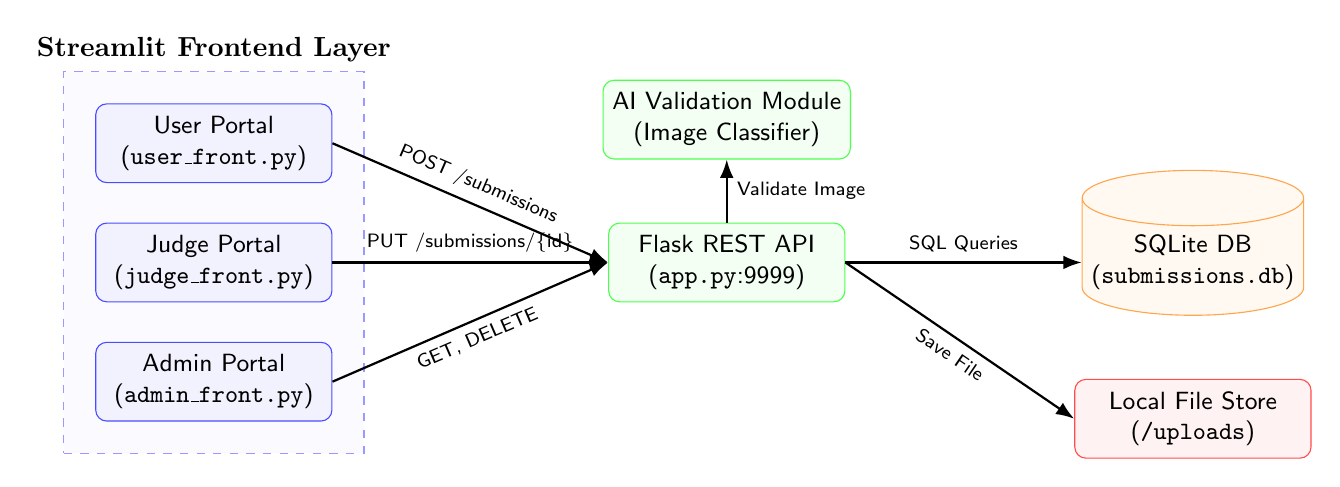
\begin{tikzpicture}[
    node distance=1.5cm and 2cm,
    block/.style={rectangle, draw=blue!70, fill=blue!5, rounded corners, minimum width=3cm, minimum height=1cm, align=center, font=\sffamily\small},
    backend/.style={rectangle, draw=green!70, fill=green!5, rounded corners, minimum width=3cm, minimum height=1cm, align=center, font=\sffamily\small},
    db/.style={cylinder, draw=orange!70, fill=orange!5, shape border rotate=90, aspect=0.25, minimum width=2.2cm, minimum height=1.2cm, align=center, font=\sffamily\small},
    line/.style={draw, -Latex, thick, font=\sffamily\scriptsize}
]

% Frontend Nodes
\node[block] (user) {User Portal\\(\texttt{user\_front.py})};
\node[block, below=0.5cm of user] (judge) {Judge Portal\\(\texttt{judge\_front.py})};
\node[block, below=0.5cm of judge] (admin) {Admin Portal\\(\texttt{admin\_front.py})};

% Subsystem Box Frontend
\begin{scope}[on background layer]
    \node[draw=blue!40, fill=blue!2, dashed, fit=(user) (judge) (admin), inner sep=0.4cm, label=above:\textbf{Streamlit Frontend Layer}] (fe_box) {};
\end{scope}

% Backend Nodes
\node[backend, right=3.5cm of judge] (api) {Flask REST API\\(\texttt{app.py}:9999)};
\node[backend, above=0.8cm of api] (ai) {AI Validation Module\\(Image Classifier)};

% Storage Nodes
\node[db, right=3cm of api] (database) {SQLite DB\\(\texttt{submissions.db})};
\node[block, draw=red!70, fill=red!5, below=0.8cm of database] (storage) {Local File Store\\(\texttt{/uploads})};

% Connections
\path [line] (user.east) -- node[above, sloped] {POST /submissions} (api.west);
\path [line] (judge.east) -- node[above, sloped] {PUT /submissions/\{id\}} (api.west);
\path [line] (admin.east) -- node[below, sloped] {GET, DELETE} (api.west);

\path [line] (api.north) -- node[right] {Validate Image} (ai.south);
\path [line] (api.east) -- node[above] {SQL Queries} (database.west);
\path [line] (api.east) -- node[below, sloped] {Save File} (storage.west);

\end{tikzpicture}
\caption{System Architecture Diagram}
\label{fig:sys_arch}
\end{figure}

\section{Database Design (Entity-Relationship Diagram)}
The relational schema comprises three main entities: \texttt{USERS}, \texttt{SUBMISSIONS}, and \texttt{EVALUATIONS}.

\begin{figure}[H]
\centering
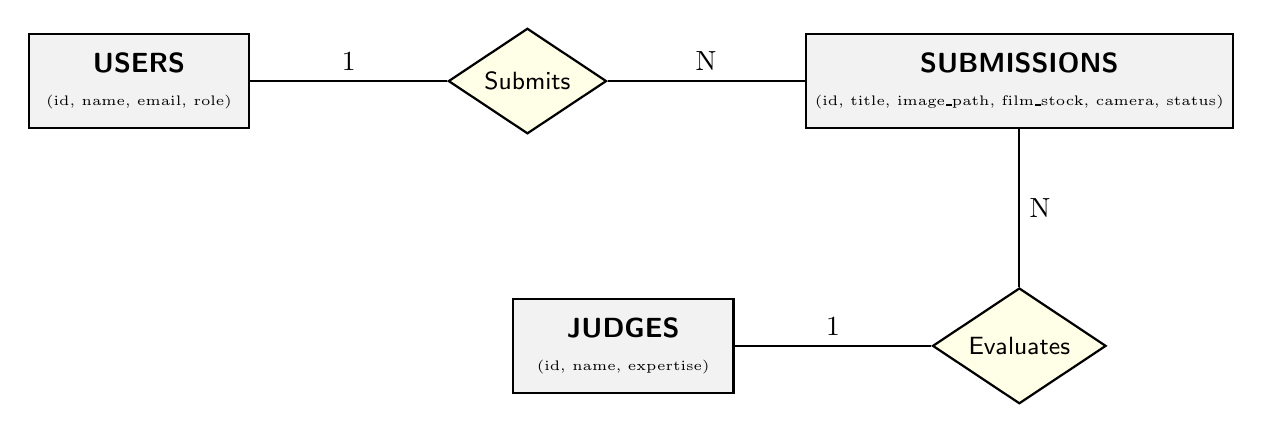
\begin{tikzpicture}[
    entity/.style={rectangle, draw=black, fill=gray!10, thick, minimum width=2.8cm, minimum height=1.2cm, align=center, font=\sffamily\bfseries},
    relationship/.style={diamond, draw=black, fill=yellow!10, thick, aspect=1.5, minimum width=2cm, align=center, font=\sffamily\small},
    line/.style={draw, thick}
]

% Entities
\node[entity] (user) {USERS\\{\normalfont\tiny (id, name, email, role)}};
\node[relationship, right=2.5cm of user] (submits) {Submits};
\node[entity, right=2.5cm of submits] (submission) {SUBMISSIONS\\{\normalfont\tiny (id, title, image\_path, film\_stock, camera, status)}};
\node[relationship, below=2cm of submission] (evaluates) {Evaluates};
\node[entity, left=2.5cm of evaluates] (judge) {JUDGES\\{\normalfont\tiny (id, name, expertise)}};

% Connections
\path [line] (user) -- node[above] {1} (submits);
\path [line] (submits) -- node[above] {N} (submission);
\path [line] (judge) -- node[above] {1} (evaluates);
\path [line] (evaluates) -- node[right] {N} (submission);

\end{tikzpicture}
\caption{Entity-Relationship Diagram (ERD)}
\label{fig:erd}
\end{figure}

\section{Sequence Diagram: Submission Workflow}
The sequence below illustrates client-side image compression followed by asynchronous REST interaction with the Flask Backend.

\begin{figure}[H]
\centering
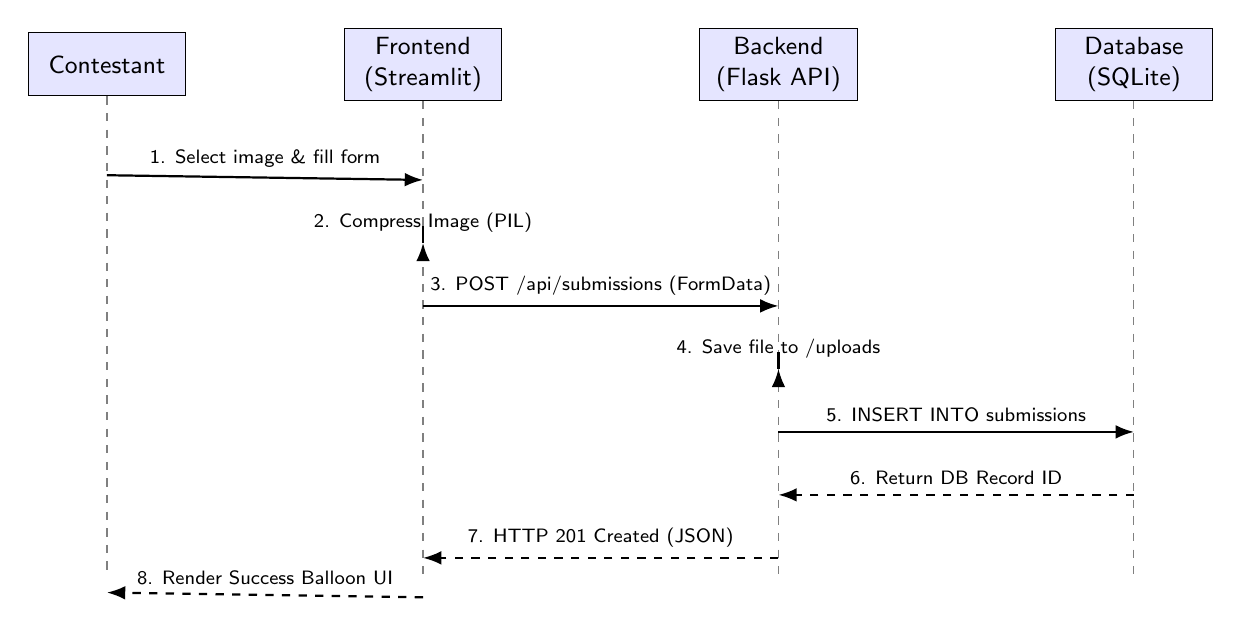
\begin{tikzpicture}[
    actor/.style={rectangle, draw, fill=blue!10, minimum width=2cm, minimum height=0.8cm, align=center, font=\sffamily\small},
    lifeline/.style={draw, dashed, gray},
    msg/.style={draw, -Latex, thick, font=\sffamily\scriptsize},
    reply/.style={draw, -Latex, dashed, thick, font=\sffamily\scriptsize}
]

% Lifeline Headers
\node[actor] (c) {Contestant};
\node[actor, right=2cm of c] (fe) {Frontend\\(Streamlit)};
\node[actor, right=2.5cm of fe] (be) {Backend\\(Flask API)};
\node[actor, right=2.5cm of be] (db) {Database\\(SQLite)};

% Vertical Lifelines
\draw[lifeline] (c) -- ++(0,-6.5);
\draw[lifeline] (fe) -- ++(0,-6.5);
\draw[lifeline] (be) -- ++(0,-6.5);
\draw[lifeline] (db) -- ++(0,-6.5);

% Messages
\draw[msg] ([yshift=-1cm]c.south) -- node[above] {1. Select image \& fill form} ([yshift=-1cm]fe.south);
\draw[msg] ([yshift=-1.8cm]fe.south) -- node[above] {2. Compress Image (PIL)} ([yshift=-1.8cm]fe.south);
\draw[msg] ([yshift=-2.6cm]fe.south) -- node[above] {3. POST /api/submissions (FormData)} ([yshift=-2.6cm]be.south);

\draw[msg] ([yshift=-3.4cm]be.south) -- node[above] {4. Save file to /uploads} ([yshift=-3.4cm]be.south);
\draw[msg] ([yshift=-4.2cm]be.south) -- node[above] {5. INSERT INTO submissions} ([yshift=-4.2cm]db.south);
\draw[reply] ([yshift=-5.0cm]db.south) -- node[above] {6. Return DB Record ID} ([yshift=-5.0cm]be.south);

\draw[reply] ([yshift=-5.8cm]be.south) -- node[above] {7. HTTP 201 Created (JSON)} ([yshift=-5.8cm]fe.south);
\draw[reply] ([yshift=-6.3cm]fe.south) -- node[above] {8. Render Success Balloon UI} ([yshift=-6.3cm]c.south);

\end{tikzpicture}
\caption{Sequence Diagram for Image Submission}
\label{fig:seq_diagram}
\end{figure}
\section{Database Design (Entity-Relationship Diagram)}
The SQLite database consists of three main entities: \texttt{USERS}, \texttt{SUBMISSIONS}, and \texttt{EVALUATIONS}. The diagram below illustrates the relational table structures, primary keys (PK), foreign keys (FK), and their cardinality relationships.

\begin{figure}[H]
\centering
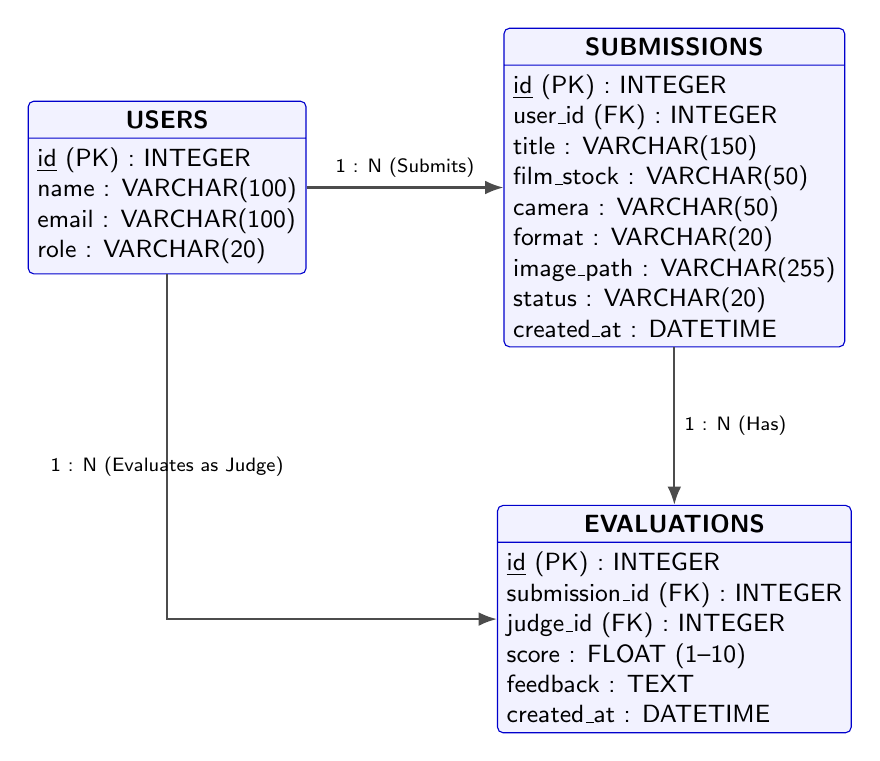
\begin{tikzpicture}[
    node distance=2.5cm and 2cm,
    table/.style={
        rectangle split,
        rectangle split parts=2,
        draw=blue!80!black,
        fill=blue!5,
        rounded corners=2pt,
        minimum width=3.5cm,
        font=\sffamily\small,
        align=left
    },
    tableheader/.style={fill=blue!20, font=\sffamily\bfseries\small},
    line/.style={draw=black!70, -Latex, thick, font=\sffamily\scriptsize}
]

% USERS Table
\node[table] (users) {
    \textbf{USERS}
    \nodepart{second}
    \underline{id} (PK) : INTEGER \\
    name : VARCHAR(100) \\
    email : VARCHAR(100) \\
    role : VARCHAR(20)
};

% SUBMISSIONS Table
\node[table, right=2.5cm of users] (submissions) {
    \textbf{SUBMISSIONS}
    \nodepart{second}
    \underline{id} (PK) : INTEGER \\
    user\_id (FK) : INTEGER \\
    title : VARCHAR(150) \\
    film\_stock : VARCHAR(50) \\
    camera : VARCHAR(50) \\
    format : VARCHAR(20) \\
    image\_path : VARCHAR(255) \\
    status : VARCHAR(20) \\
    created\_at : DATETIME
};

% EVALUATIONS Table
\node[table, below=2cm of submissions] (evaluations) {
    \textbf{EVALUATIONS}
    \nodepart{second}
    \underline{id} (PK) : INTEGER \\
    submission\_id (FK) : INTEGER \\
    judge\_id (FK) : INTEGER \\
    score : FLOAT (1--10) \\
    feedback : TEXT \\
    created\_at : DATETIME
};

% Relationships / Connectors
\path[line] (users.east) -- node[above] {1 : N (Submits)} (submissions.west);
\path[line] (submissions.south) -- node[right] {1 : N (Has)} (evaluations.north);
\path[line] (users.south) |- node[below, near start] {1 : N (Evaluates as Judge)} (evaluations.west);

\end{tikzpicture}
\caption{Entity-Relationship Diagram (Database Relational Schema)}
\label{fig:erd_detailed}
\end{figure}
\chapter{API Specification}

\section{Endpoint Summary}
The Flask API communicates over standard HTTP protocols, accepting form-data and returning JSON payloads.

\begin{table}[h!]
\centering
\renewcommand{\arraystretch}{1.4}
\begin{tabular}{|l|l|p{6cm}|}
\hline
\textbf{HTTP Method} & \textbf{Endpoint Path} & \textbf{Functional Description} \\ \hline
\texttt{POST} & \texttt{/api/submissions} & Accepts submission metadata and image file. \\ \hline
\texttt{GET} & \texttt{/api/submissions} & Retrieves all submissions with scores. \\ \hline
\texttt{PUT} & \texttt{/api/submissions/\{id\}} & Updates score and evaluation notes. \\ \hline
\texttt{DELETE} & \texttt{/api/submissions/\{id\}} & Deletes an entry from DB and filesystem. \\ \hline
\end{tabular}
\caption{API Endpoints Overview}
\end{table}

\section{Sample Payloads}

\subsection{POST /api/submissions Request}
Multipart form-data fields:
\begin{itemize}
    \item \texttt{name}: "Jane Doe"
    \item \texttt{title}: "Sunset on Kodak Gold"
    \item \texttt{film\_stock}: "Kodak Gold 200"
    \item \texttt{camera}: "Leica M6"
    \item \texttt{file}: Binary image data (JPEG)
\end{itemize}

\subsection{Response (201 Created)}
\begin{verbatim}
{
  "status": "success",
  "message": "Submission created successfully",
  "data": {
    "id": 102,
    "title": "Sunset on Kodak Gold",
    "image_path": "/uploads/102_sunset.jpg"
  }
}
\end{verbatim}
\chapter{UI/UX Design \& User Manual}

\section{UI Design Principles}
The interfaces are built using Streamlit with a dark theme optimized for viewing photography:
\begin{itemize}
    \item \textbf{User Portal:} Single-column form structure with clear upload status and warning indicators.
    \item \textbf{Judge Portal:} Grid-based layout displaying high-resolution photos alongside metadata cards and score sliders.
    \item \textbf{Admin Portal:} Dashboard layout with summary metrics and editable data tables.
\end{itemize}

\section{User Manual}

\subsection{Submitting an Entry (Contestant)}
\begin{enumerate}
    \item Open the User Portal in a browser.
    \item Fill in contestant information (Name, Artwork Title, Film Stock, Camera).
    \item Click \textbf{Browse files} to select a film photo (PNG, JPG, WEBP).
    \item Click \textbf{Submit}. Client-side compression executes automatically before sending data to the server.
\end{enumerate}

\subsection{Grading Entries (Judge)}
\begin{enumerate}
    \item Open the Judge Portal.
    \item Select an ungraded photo from the list.
    \item Review image details and EXIF metadata.
    \item Adjust the score slider (1--10), enter comments, and click \textbf{Save Evaluation}.
\end{enumerate}
\chapter{Software Testing}

\section{Test Strategy}
Testing focuses on verifying image compression efficiency, API response correctness, and database consistency.

\section{Test Cases}
\begin{table}[h!]
\centering
\renewcommand{\arraystretch}{1.3}
\begin{tabular}{|c|p{4.5cm}|p{4.5cm}|c|}
\hline
\textbf{Test ID} & \textbf{Action / Input} & \textbf{Expected Outcome} & \textbf{Status} \\ \hline
TC-01 & Submit form with empty "Name" field. & UI displays missing field warning; API call blocked. & PASS \\ \hline
TC-02 & Upload 3.7MB photo file. & Client compresses image to <300KB and POST succeeds (201). & PASS \\ \hline
TC-03 & Judge submits valid score (8/10). & DB updates score field; entry disappears from ungraded queue. & PASS \\ \hline
TC-04 & Admin triggers DELETE request. & Database record and local image file are both removed. & PASS \\ \hline
\end{tabular}
\caption{System Test Cases}
\end{table}
\chapter{Deployment \& Conclusion}

\section{System Deployment}

\subsection{Prerequisites}
Python 3.9+ environment with required packages installed via:
\begin{verbatim}
pip install -r requirements.txt
\end{verbatim}

\subsection{Execution Steps}
\begin{enumerate}
    \item Start Backend API: \texttt{python src/app.py} (Port 9999).
    \item Launch Admin Portal: \texttt{streamlit run admin\_front.py --server.port 8501} (Port 8501).
    \item Launch Judge Portal: \texttt{streamlit run judge\_front.py --server.port 8502} (Port 8502).
    \item Launch User Portal: \texttt{streamlit run user\_front.py --server.port 8503} (Port 8503).
\end{enumerate}

\section{Conclusion \& Future Work}
\begin{itemize}
    \item \textbf{Conclusion:} The system successfully digitalizes film photography submission and judging workflows. Client-side compression effectively eliminates network timeouts caused by large photo files.
    \item \textbf{Future Work:} Implement JWT user authentication, deploy cloud storage for uploaded assets (e.g., AWS S3), and train a custom vision model for automated film border detection.
\end{itemize}

\end{document}
